\section{Additional Budget-Curve Figures}
\label{app:budget-curves}

Figures~\ref{fig:openthoughts_budget_pass_rates_thinking5_fs_ao}
and~\ref{fig:openthoughts_budget_response_lengths_thinking5_fs_ao} split the
budget-dependent results in Figure~\ref{fig:openthoughts_accuracy_length_collapse}
into pass-rate and response-length views across the five thinking models in
Table~\ref{tab:openthoughts_thinking_models}.
Figure~\ref{fig:openthoughts_qwen8b_concise_budget} adds a conciseness-prompt
comparison for \qweneightb{}.
Figure~\ref{fig:qwen17_opd_gold_demo_budget_curves} gives the corresponding
budget-curve view for the context-enhanced OPD comparison in
Table~\ref{tab:qwen17_openthoughts_opsd_opd}.

\paragraph{Relation to CRISP-style reasoning compression.}
CRISP \citep{sang2026policy} studies a complementary setting in which the
teacher is conditioned on a conciseness instruction rather than on a gold answer
or reference solution. Thus, unlike gold-context \opsd{}, CRISP does not give
the teacher task-answer information, but its token-level supervision can still
act globally across the rollout: the teacher is encouraged to prefer shorter,
more direct continuations at many positions. Our Qwen3-8B conciseness-prompt
control confirms the first-order CRISP effect, namely that such conditioning
shortens responses. However, the comparison with final-answer-only and
full-demonstration \opsd{} shows that response shortening is not unique to
conciseness distillation. Dense gold-demonstration context produces the
strongest long-budget compression, while final-answer-only context remains
closer to the base model. Thus, our claim is not that compression itself is
always harmful, but that token-level teachers which broadly suppress
deliberative continuations can remove the long-budget gains of thinking models.

\begin{figure}[!htbp]
    \centering
    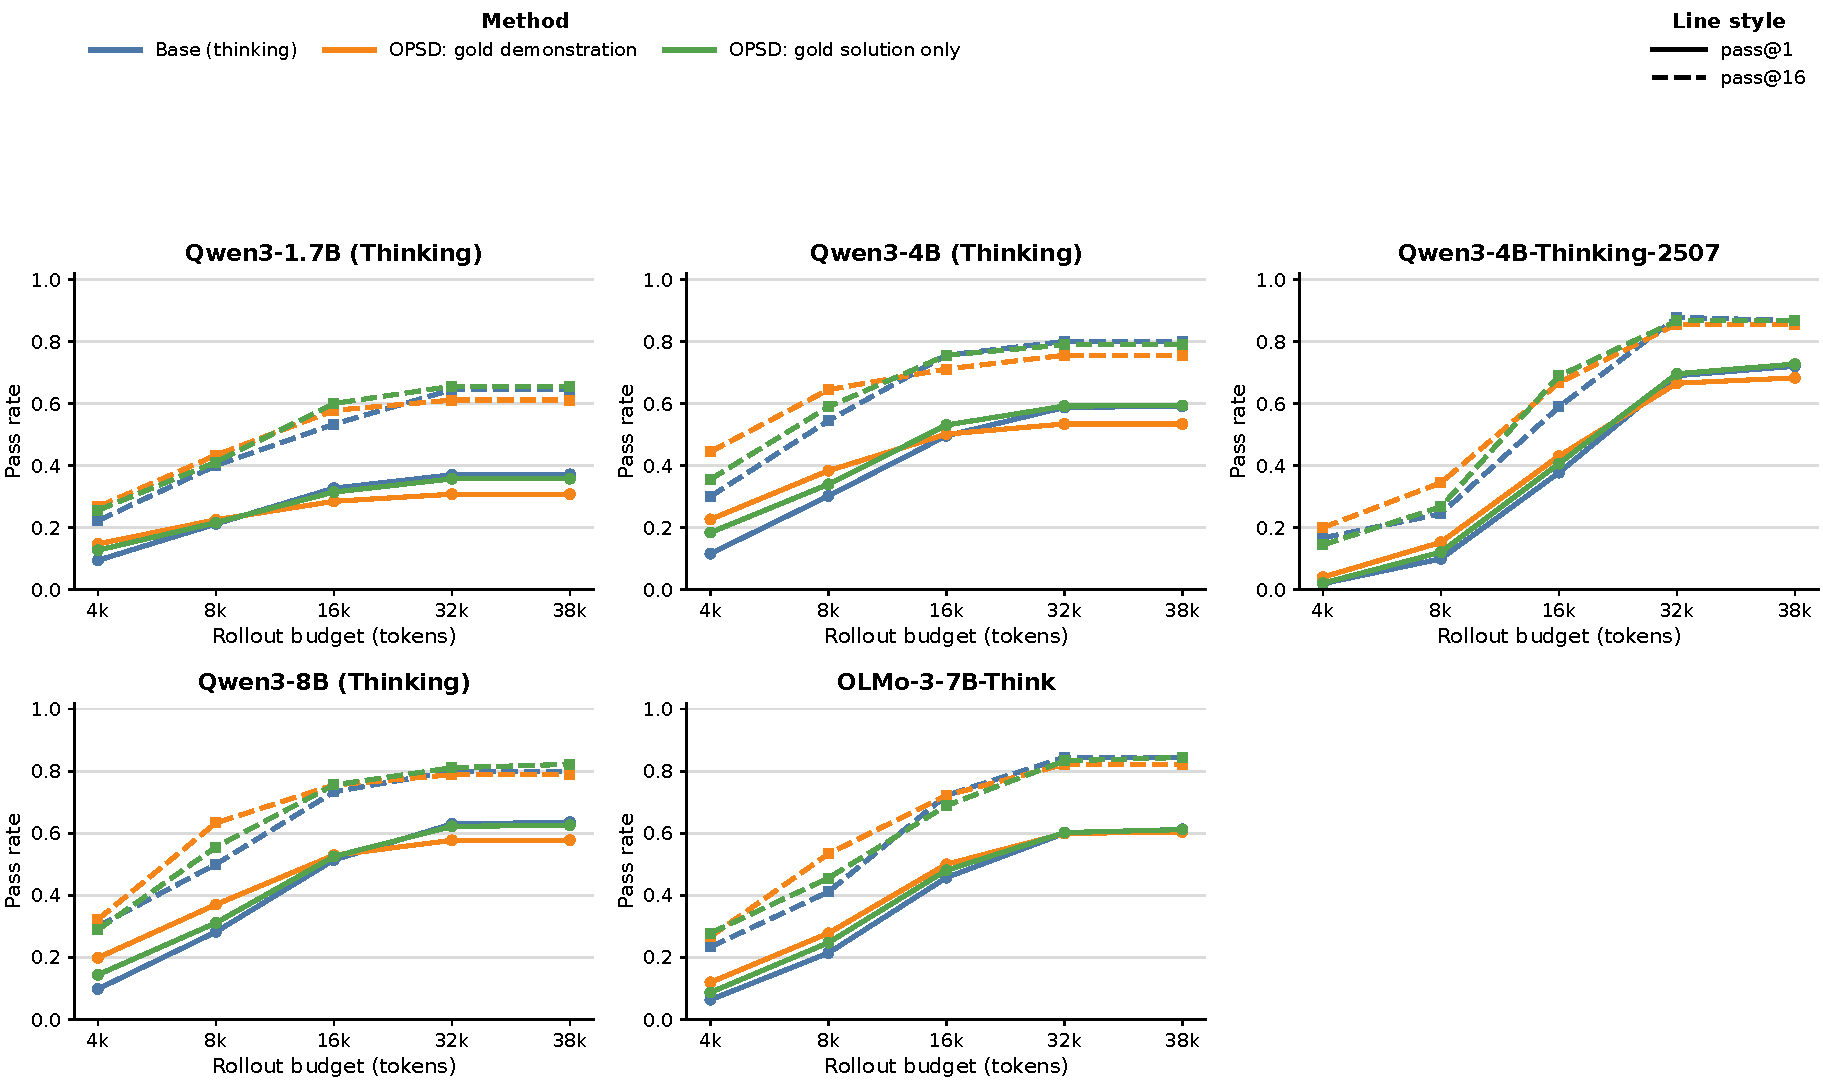
\includegraphics[width=\linewidth]{figures/avg_pass_budget_curves_thinking5_fs_ao.pdf}
    \caption{
    \textbf{Per-model pass-rate budget curves separate the accuracy effects in Figure~\ref{fig:openthoughts_accuracy_length_collapse}.}
    We evaluate five OpenThoughts-trained thinking models at rollout budgets from 4k to 38k tokens on AIME24, AIME25, and HMMT25.
    Solid lines show pass@1 and dashed lines show pass@16.
    Blue curves are base thinking models, orange curves are \opsd{} with full gold-demonstration context, and green curves are \opsd{} with final-answer-only privileged context.
    Dense demonstrations tend to give larger short-budget gains, while the advantage narrows or reverses at longer budgets for several models.
    }
    \label{fig:openthoughts_budget_pass_rates_thinking5_fs_ao}
\end{figure}


\begin{figure}[!htbp]
    \centering
    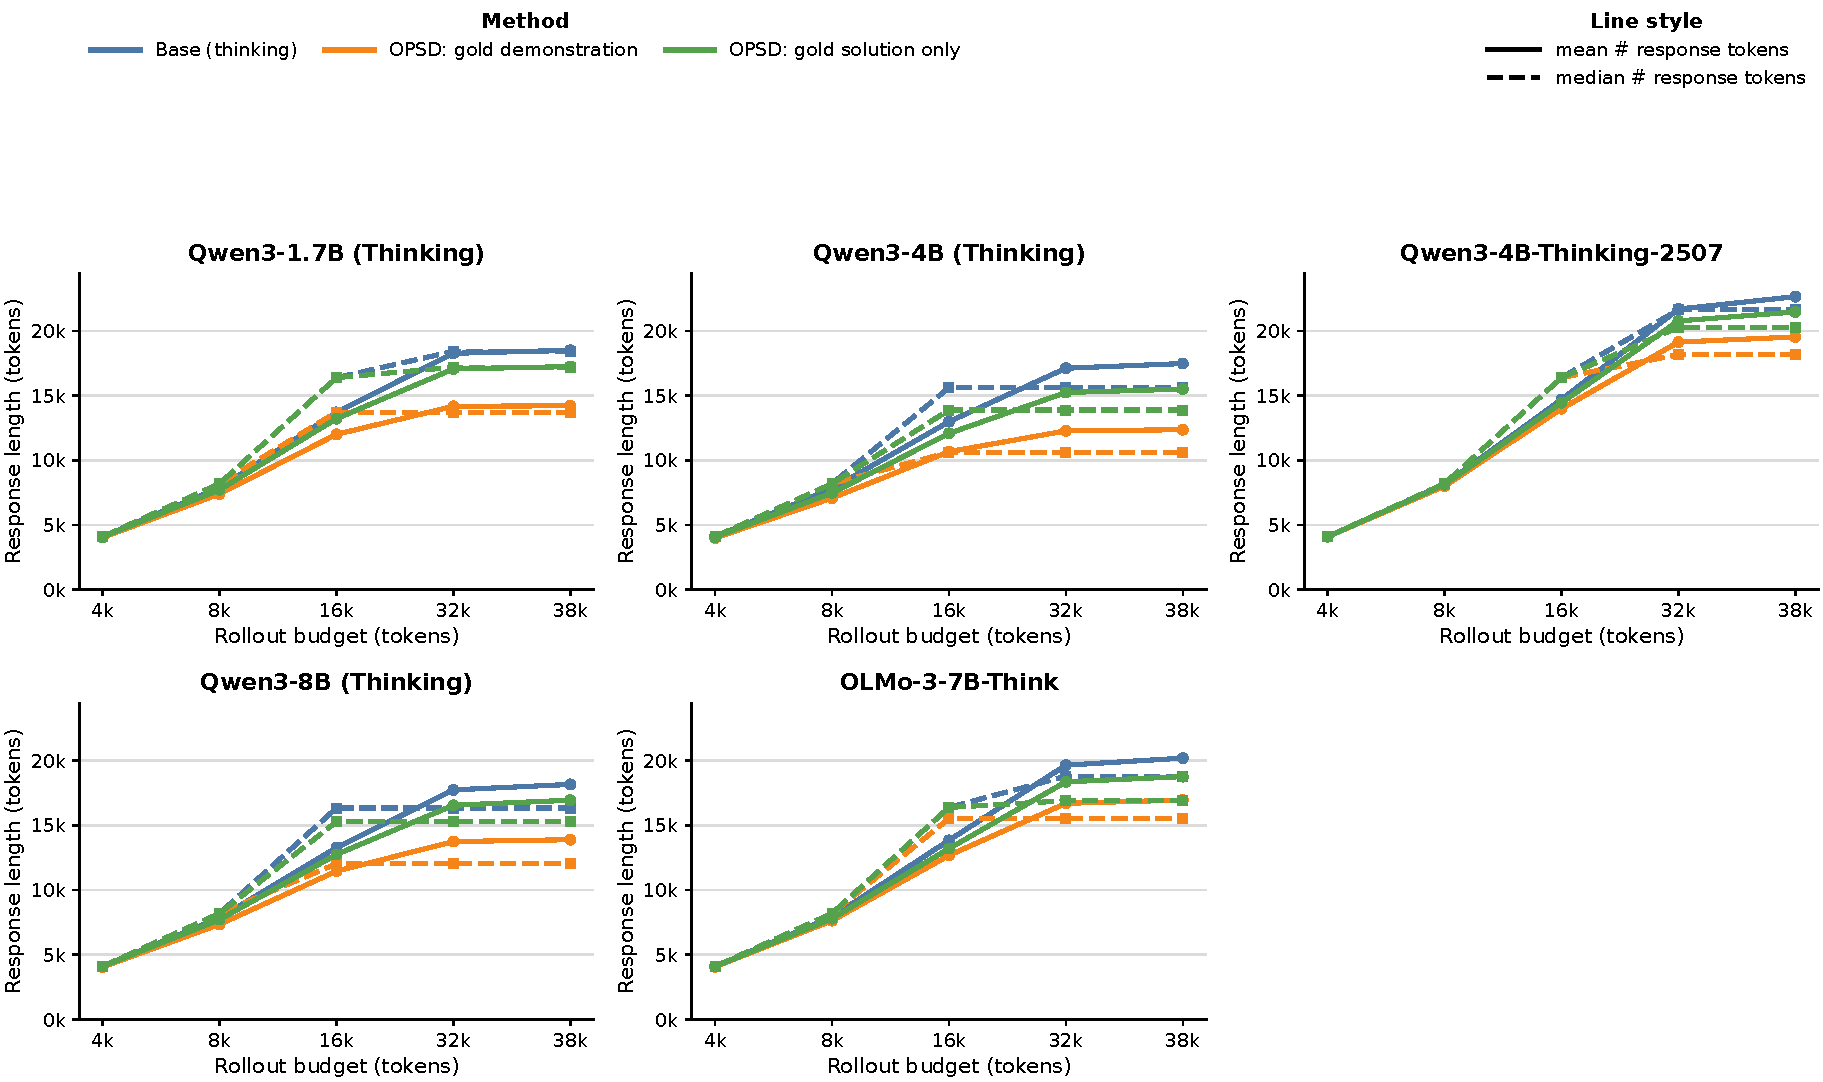
\includegraphics[width=\linewidth]{figures/avg_rollout_tokens_budget_curves_thinking5_fs_ao.pdf}
    \caption{
    \textbf{Per-model response-length budget curves show where \opsd{} compresses long thinking rollouts.}
    This companion to Figure~\ref{fig:openthoughts_accuracy_length_collapse} reports response-token counts for the same five OpenThoughts-trained thinking models, evaluation benchmarks, and rollout budgets as Figure~\ref{fig:openthoughts_budget_pass_rates_thinking5_fs_ao}.
    Solid lines show mean response length and dashed lines show median response length.
    Blue curves are base thinking models, orange curves are \opsd{} with full gold-demonstration context, and green curves are \opsd{} with final-answer-only privileged context.
    At 32k--38k token budgets, full-demonstration \opsd{} generally produces shorter responses than the corresponding base model.
    }
    \label{fig:openthoughts_budget_response_lengths_thinking5_fs_ao}
\end{figure}


\begin{figure}[!htbp]
    \centering
    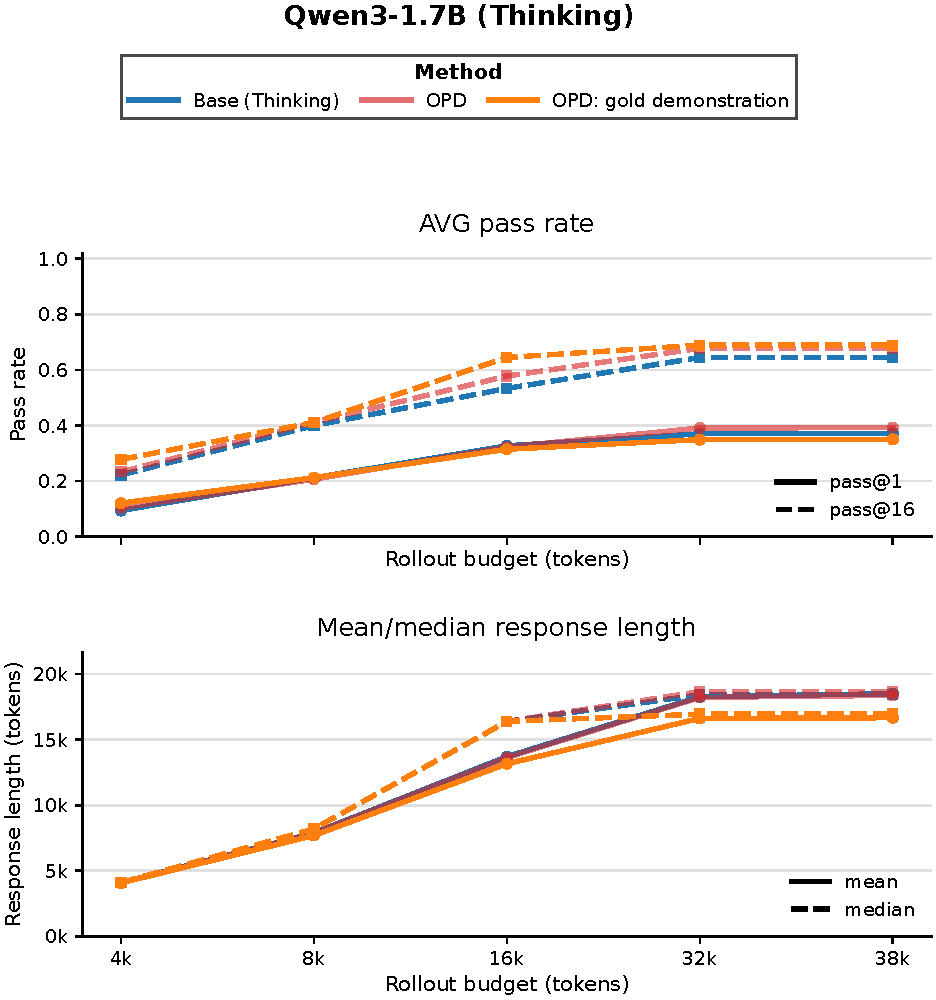
\includegraphics[width=\linewidth]{figures/avg_pass_rollout_tokens_qwen_1p7b_thinking_opd_gold_demo.pdf}
    \caption{
    \textbf{OPD with gold-demonstration context shortens response lengths while vanilla OPD preserves the base length profile.}
    This budget-curve companion to Table~\ref{tab:qwen17_openthoughts_opsd_opd} evaluates the \qwenonesevenb{} thinking student with a larger \qweneightb{} teacher.
    We compare the base model, vanilla OPD, and OPD with gold-demonstration teacher context.
    The OPD variants are trained with a 4,096-token completion cap, and all methods are evaluated at generation caps from 4,096 to 38,912 tokens.
    Top row: pass@1 and pass@16, averaged over AIME24, AIME25, and HMMT25.
    Bottom row: mean and median response length.
    Vanilla OPD mildly improves pass@k while largely preserving the base model's response-length curve.
    Adding gold-demonstration context to the teacher shortens responses and reduces the pass@1 gains; its long-budget degradation is milder than in the \opsd{} setting, consistent with the use of a stronger larger teacher.
    }
    \label{fig:qwen17_opd_gold_demo_budget_curves}
\end{figure}


\begin{figure}[!htbp]
    \centering
    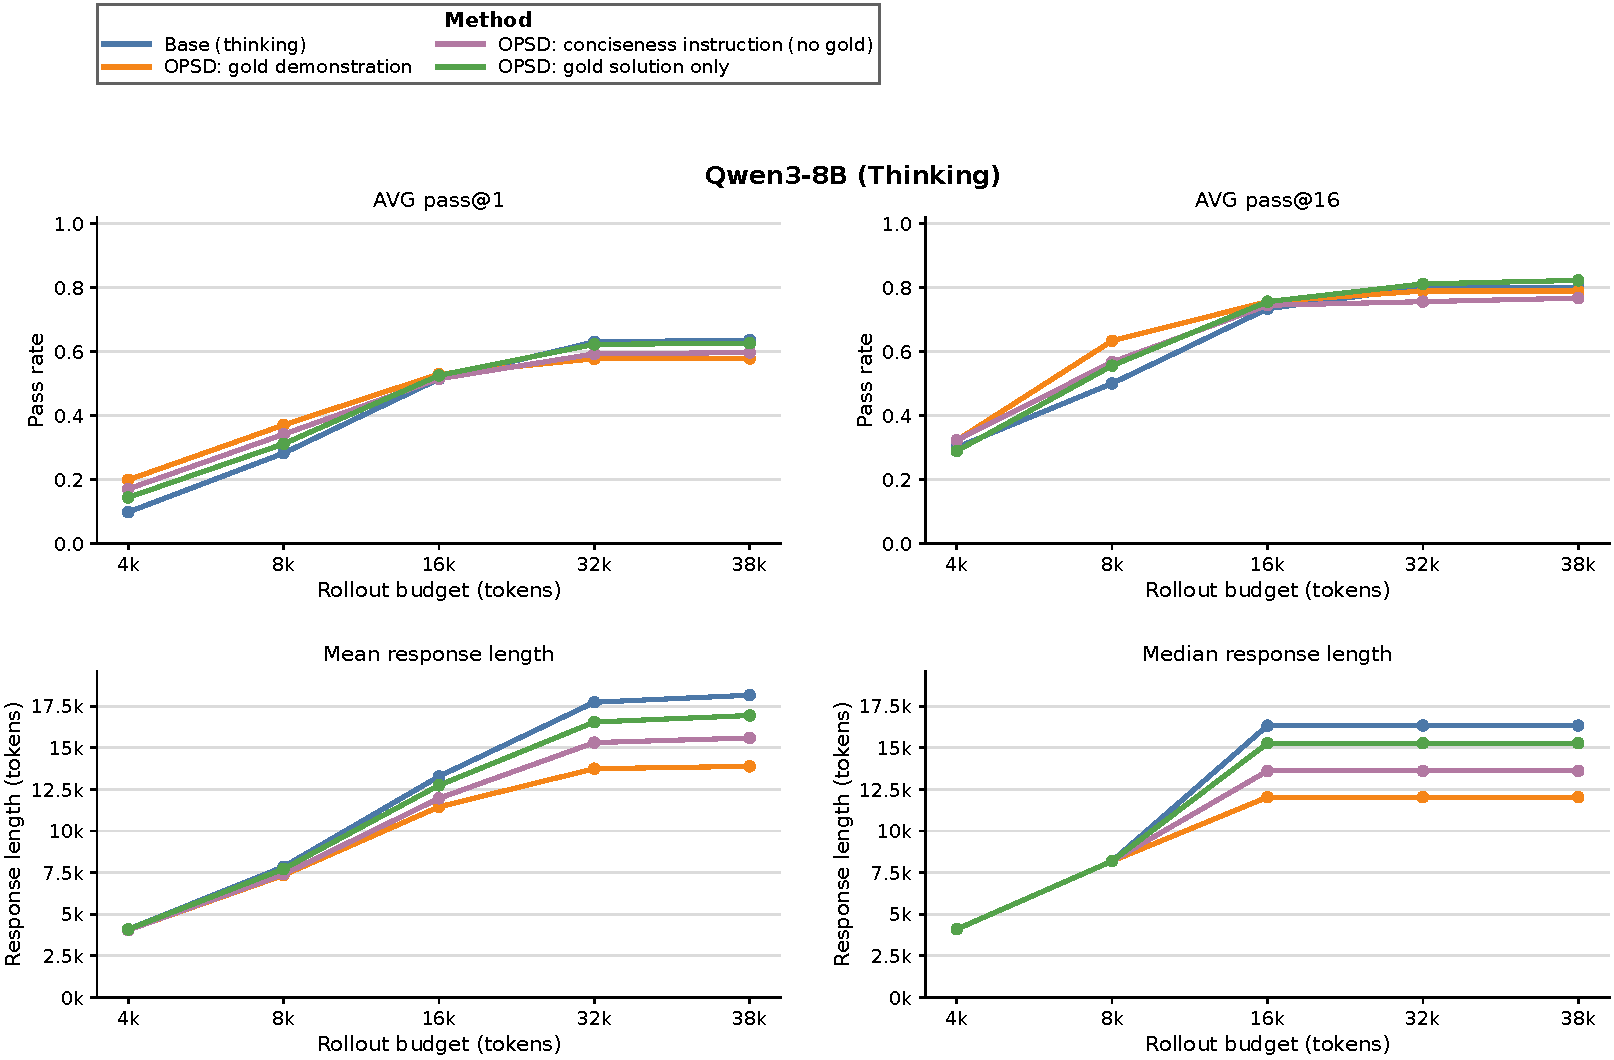
\includegraphics[width=\linewidth]{figures/avg_pass_rollout_qwen8b_with_concise.pdf}
    \caption{
    \textbf{A CRISP-style conciseness prompt compresses Qwen3-8B responses but does not recover the long-budget gains.}
    We compare base \qweneightb{} thinking, \opsd{} with full gold demonstrations, \opsd{} with final-answer-only privileged context, and a conciseness-instruction condition with no gold context, following the CRISP prompt direction of \citep{sang2026policy}.
    Top panels report pass@1 and pass@16 averaged over AIME24, AIME25, and HMMT25; bottom panels report mean and median response length.
    The conciseness condition shortens 32k--38k rollouts relative to the base and gold-solution-only runs but is less compressive than full gold demonstrations.
    Its accuracy follows the same tradeoff: it improves short-budget performance but, at long budgets, remains below the base and gold-solution-only curves, suggesting that making the student concise alone is not enough to preserve the gains from longer thinking rollouts.
    }
    \label{fig:openthoughts_qwen8b_concise_budget}
\end{figure}

